\documentclass[%
 reprint,
%superscriptaddress,
%groupedaddress,
%unsortedaddress,
%runinaddress,
%frontmatterverbose, 
%preprint,
%preprintnumbers,
%nofootinbib,
%nobibnotes,
%bibnotes,
 amsmath,amssymb,
 aps,
%pra,
%prb,
%rmp,
%prstab,
%prstper,
%floatfix,
]{revtex4-2}

\usepackage{graphicx}% Include figure files
\usepackage{dcolumn}% Align table columns on decimal point
\usepackage{bm}% bold math
%\usepackage{hyperref}% add hypertext capabilities
%\usepackage[mathlines]{lineno}% Enable numbering of text and display math
%\linenumbers\relax % Commence numbering lines

%\usepackage[showframe,%Uncomment any one of the following lines to test 
%%scale=0.7, marginratio={1:1, 2:3}, ignoreall,% default settings
%%text={7in,10in},centering,
%%margin=1.5in,
%%total={6.5in,8.75in}, top=1.2in, left=0.9in, includefoot,
%%height=10in,a5paper,hmargin={3cm,0.8in},
%]{geometry}
\usepackage[version=4]{mhchem}%nombres compuestos quimicos
\usepackage{textcomp}%Para angulos
%%%%%%%%%%%%%%%%%%%%%%%%%%%%%%%%%%%%%%%%%%%%%%%%%%%%%%%%%%%%%%%%%%
\begin{document}

\preprint{APS/123-QED}
\title{Estudio del Comportamineto Termodin\'{a}mico de \textit{Staphyloccocus aureus} por la T\'{e}cnica FTIR}% Force line breaks with \\
%\title{Manuscript Title:\\with Forced Linebreak}% Force line breaks with \\
%\thanks{A footnote to the article title}%


\author{John Erick Cabrera Ramirez}
\affiliation{
Universidad de los Andes\\
 \email{je.cabrera@uniandes.edu.co}
}

%\collaboration{CLEO Collaboration}%\noaffiliation

\date{\today}% It is always \today, today,
             %  but any date may be explicitly specified

\begin{abstract}
\begin{center}
  \textit{Resumen}  
\end{center}
Se estudia la transici\'{o}n de fase s\'{o}lido ordenado a l\'{i}quido desordenado  en 1) membranas modelo DMPC, 2) en membranas de \textit{Staphyloccocus aureus} en presencia de estafiloxantina y 3) en ausencia de estafiloxantina. La transici\'{o}n de fase se estudia usando la t\'{e}cnica FTIR y se determina mediante el cambio termotr\'{o}pico del n\'{u}mero de onda de la banda de absorci\'{o}n \ce{CH_{2}} de los \'{a}cidos grasos. 1) Para membranas de DMPC se encuentra una temperatura de transici\'{o}n de $T_{1}=(22\pm2)$\textdegree C. Para membranas de \textit{Staphylococcus aureus} , primero se realizan curvas de crecimiento de tres cepas, una cepa nativa 2), una mutante que no produce estafiloxantina  3) y una  complementada que produce carotenoides. La cepa nativa 2), la mutante 3) y la complementada llegan a la fase estacionaria a $t_{n}=(22\pm2)$h, $ t_{m} =(22\pm2)$h y $ t_{c}= (22\pm2)$h respectivamente. De las cepas nativa y mutante se forman membranas con l\'{i}pidos y carotenoides y llevan al FTIR. Para las cepas nativa y mutante se obtiene una temperatura de transici\'{o}n de $T_{2}=(22\pm2)$\textdegree C y $T_{3}=(22\pm2)$\textdegree C respectivamente. Debido a la diferencia entre las dos temperaturas, existe cooperatividad en la transici\'{o}n de fase.
%Se estudian cambios en la transici\'{o}n de fase s\'{o}lido ordenado a l\'{i}quido desordenado  en 1) membranas modelo DMPC y 2) en membranas de \textit{Staphyloccocus aureus} en presencia del carotenoide estafiloxantina y 3) membranas de \textit{Staphyloccocus aureus} en ausencia de estafiloxantina. La transici\'{o}n de fase se estudia usando la t\'{e}cnica de espectrofotometr\'{i}a infrarroja por transformada de Fourier (FTIR) y se determina mediante el aumento del n\'{u}mero de onda de la banda de absorci\'{o}n \ce{CH_{2}} de los \'{a}cidos grasos en funci\'{o}n de la temperatura. 1) Para membranas de DMPC preparadas y proporcionadas por el grupo de biof\'{i}sica de la Universidad de los Andes, se encuentra una temperatura de transici\'{o}n de $T_{1}=(22\pm2)$\textdegree C. Para las membranas de \textit{Staphylococcus aureus}, casos 2) y 3)  antes de medir los espectros se realizan curvas de crecimiento de \textit{Staphylococcus aureus} para tres cepas, una cepa nativa (caso 2)), una que es un mutante  del gen crtM de la ruta de s\'{i}ntesis de estafiloxantina (caso 3)) y una variante  complementada con pl\'{a}smido que contiene crtMN la cual produce un exceso de carotenoides. La cepa nativa 2), la mutante 3) y la complementada llegan a la fase estacionaria en los tiempos $(22\pm2)$h, $(22\pm2)$h y $(22\pm2)$h respectivamente. De las cepas nativa 2) y mutante 3) se extraen l\'{i}pidos y carotenoides, se forman membranas las cuales se llevan al FTIR para el seguimiento de la banda de \ce{CH_{2}} en funci\'{o}n de la temperatura. Para las cepas nativa 2) y mutante 3) se obtiene una temperatura de transici\'{o}n de $T_{2}=(22\pm2)$\textdegree C y $T_{3}=(22\pm2)$\textdegree C respectivamente. Debido a la diferencia entre las dos temperaturas, existe un nivel de cooperatividad de la transici\'{o}n de fase.
\end{abstract}

\keywords{}%Use showkeys class option if keyword
                              %display desired
\maketitle

%\tableofcontents

\section{\label{sec:intro}Introducci\'{o}n y Estado del Arte}
%\subsection{\textit{S. Aureus} y su Membrana}
\textit{Staphylococcus aureus} es una bacteria pat\'{o}gena (que causa enfermedades infecciosas) tipo Gram-positiva,  la cual se encuentra en la microbiota humana sin producir enfermedades en condiciones normales, pero que en condiciones desfavorables tales como heridas y cicatrices operatorias puede causar o estar relacionada con enfermedades de diferente gravedad en el sistema respiratorio, en los tejidos blandos y en el torrente sangu\'{i}neo \cite{1HarpavatS.NissimS.LipppincottsMicrocards:MicrobiologyFlashCards2012.}.\\
%\begin{figure}[h]
 % 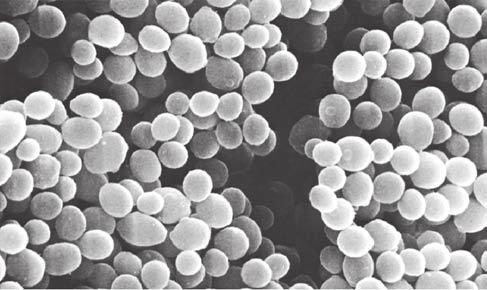
\includegraphics[width=\linewidth]{s_aureus.jpg}
  %\caption{Fotograf\'{i}a  de \textit{Staphylococcus aureus}. Tomado de \cite{1HarpavatS.NissimS.LipppincottsMicrocards:MicrobiologyFlashCards2012.}}
%  \label{fig:sta}
%\end{figure}

Desde el descubrimiento de \textit{S. aureus} como causante de una infecci\'{o}n a una herida en 1881 \cite{Orent2006AMagazine}, se ha investigado su presencia en otras infecciones y se han utilizado antibi\'{o}ticos como la penicilina y la meticilina para controlar estas infecciones \cite{1HarpavatS.NissimS.LipppincottsMicrocards:MicrobiologyFlashCards2012.}. Sin embargo \textit{S. aureus} ha desarrollado resistencia a estos antibi\'{o}ticos,  surgiendo la necesidad de buscar nuevos antibi\'{o}ticos, entre los cuales se encuentran los p\'{e}ptidos antimicrobianos.\\
Los p\'{e}ptidos antimicrobianos interact\'{u}an con la membrana de la bacteria produciendo orificios que causan p\'{e}rdida de contenido y muerte celular. La resistencia a los poros. Para entender como puede generar resistencia a estos antibi\'{o}ticos es importante estudiar la rigidez mec\'{a}nica y la elasticidad de la membrana. Adicionalmente, se sabe que la composici\'{o}n de la bicapa lip\'{i}dica de la membrana de \textit{S. aureus} cambia de manera adaptativa al medio ambiente, volvi\'{e}ndose m\'{a}s resistente como respuesta a estr\'{e}s externo.\\
\textit{S. aureus} al ser una bacteria Gram positiva tiene expuesto al exterior un compuesto llamado peptidoglicando. La membrana celular que recubre la bacteria es una bicapa fosfolip\'{i}dica que contiene dos capas de glicerofosfol\'{i}pidos. Los glicerofosfol\'{i}pidos son mol\'{e}culas anfip\'{a}ticas, las cuales tienen una parte hidrof\'{o}bica y otra parte hidrof\'{i}lica \cite{Nelson2011}, al ser anfip\'{a}ticas la parte interna de la bicapa es hidrof\'{o}bica mientras que la parte externa de la membrana es hidrof\'{i}lica. La interacci\'{o}n lateral entre estas mol\'{e}culas se da trav\'{e}s de fuerzas no covalentes lo que le confiere propiedades de cristal l\'{i}quido caracterizado por la capacidad de presentar transiciones de fase s\'{o}lido-l\'{i}quido. \\
La membrana de \textit{S. aureus} est\'{a} compuesta principalmente por  fosfatidiletalonamina, cardiolipina, fosfatidilglicerol y estafiloxantina \cite{Ocampo2010TheAureus}, siendo la estafiloxantina un carotenoide que le da el color dorado (a\'{u}reo) caracter\'{i}stico de \textit{S. aureus}. Adem\'{a}s, dependiendo de la composici\'{o}n espec\'{i}fica de la membrana celular dicha membrana va a ser m\'{a}s o menos r\'{i}gida lo cual implica corrimientos en la temperatura de transici\'{o}n y cambios en la cooperatividad de la transici\'{o}n de fase. La estructura molecular de los fosfol\'{i}pidos presentes en la membrana hace que esta sea m\'{a}s fluida cuando la estructura presenta mol\'{e}culas con m\'{u}ltiples insaturaciones que inducen un incremento en espaciamiento, reduciendo la interacci\'{o}n entre ellas. La membrana puede pasar de un estado s\'{o}lido-ordenado (so) a un estado l\'{i}quido-desordenado (ld) con un incremento de temperatura. En el caso de \textit{S. aureus} se ha descubierto que su membrana cambia el estado de rigidez de su membrana modulando la cantidad de estafiloxantinas presentes y la cantidad de cardiolipinas. \\
En cuanto a la fluidez de la membrana de acuerdo a la temperatura, si se estudia una membrana compuesta \'{u}nicamente por glicerofosfol\'{i}pidos, tal como se muestra en \cite{Heimburg}, esta presenta diferentes estados de acuerdo a su temperatura:  laminar l\'{i}quido cristalino, gel laminar, laminar ondulada, entre otras.

Debido a la importancia de la rigidez de la membrana lip\'{i}dica en los procesos de defensa de la c\'{e}lula e incluso para la b\'{u}squeda de nuevos antibi\'{o}ticos, el objetivo principal es estudiar la transici\'{o}n de fase s\'{o}lido-ordenado/l\'{i}quido-desordenado de la membrana de S.aureus en presencia y ausencia de estafiloxantina con base en gr\'{a}ficas de posici\'{o}n de la banda CH$_{2}$ asim\'{e}trico en funci\'{o}n de la temperatura.\\
Para enteder la transici\'{o}n de fase de una membrana en un sistema vivo, primero se estudia la transici\'{o}n fase en un sistema modelo compuesto por un solo tipo de l\'{i}pidos.
\subsection{Transiciones de Fase en L\'{i}pidos}
En soluci\'{o}n con agua, los l\'{i}pidos tienden a formar agregados debido a  su car\'{a}cter anfip\'{a}tico. Para concentraciones mucho mayores a cierta concentraci\'{o}n cr\'{i}tica \cite{Heimburg}, los l\'{i}pidos tienden a formar bicapas. Las fases de estas bicapas se conocen como fases laminares y seg\'{u}n su incremento en la temperatura se clasifican en:
\begin{itemize}
    \item \textit{Fase} $L_{c}$: Los l\'{i}pidos forman bicapas que presentan un orden en las tres dimensiones, es decir, las cabezas polares del l\'{i}pido presentan un patr\'{o}n en forma de red mientras que las cadenas apolares est\'{a}n ordenadas en configuraci\'{o}n  trans.
    \item  \textit{Fase} $L_{\beta'}$: Esta es conocida como la fase gel. En esta los l\'{i}pidos se encuentran mayoriatariamente ordenados pero no todas cadenas hidrocarbonadas son trans. Se llama $\beta'$ porque algunos l\'{i}pidos presentan una inclinaci\'{o}n respecto al plano de la normal, \cite{Heimburg}.
    \item  \textit{Fase} $P_{\beta '}$: Esta fase es una mezcla entre las fases de gel $L_{\beta '}$ y fluida $L_{\alpha}$. Se denomina as\'{i} porque la membrana presenta ondulaciones peri\'{o}dicas.
      \item  \textit{Fase} $L_{\alpha}$: Esta es la fase l\'{i}quida o fluida de la membrana donde no hay un orden lateral de los grupos polares ni en las cadenas hidrocarbonadas.
\end{itemize}
Cuando ocurre una transici\'{o}n de fase de primer orden, la presi\'{o}n y la temperatura son aproximadamente constantes. El calor espec\'{i}fico a presi\'{o}n constante se calcula mediante la relaci\'{o}n:
\begin{equation}
    c_{p}=\left(\frac{\partial H}{\partial T}\right)_{P}
\end{equation}\label{eq:1}
Donde $H$ es la entalp\'{i}a del sistema, en este caso de la membrana bacteriana. Cuando ocurre la transici\'{o}n de fase, hay un salto de la entalp\'{i}a. Cuando hay un salto en la entalp\'{i}a, el calor espec\'{i}fico $c_{p}$ presenta un pico, como una funci\'{o}n tipo aguja.\\
Para liposomas con un solo l\'{i}pido se encuentran mediante m\'{e}todos de calorimetr\'{i}a las curvas de calor espec\'{i}fico mostradas en la figura \ref{fig:esp3}. Los tres compuestos son dimiristoil fosfatidilcolina ( por sus siglas en ingl\'{e}s DMPC), dipalmitoilfosfatidilcolina ( por sus siglas en ingl\'{e}s DPPC) y diasteroilfosfatidilcolina ( por sus siglas en ingl\'{e}s DSPC).
\begin{figure}[h]
  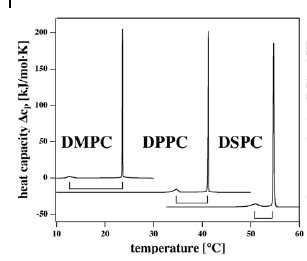
\includegraphics[width=\linewidth]{cp.png}
  \caption{ Calor espec\'{i}fico en funci\'{o}n de la temperatura para tres l\'{i}pidos diferentes. Los picos representan la transici\'{o}n de fase cada uno.Tomado de \cite{Heimburg}}.
  \label{fig:esp3}
\end{figure}
 Como la composici\'{o}n de la bicapa fosfolip\'{i}dica de \textit{S. aureus} no contiene \'{u}nicamente el mismo tipo de fosfol\'{i}pidos, sino principalmente los que se han mencionado previamente, entonces no se espera obtener una transici\'{o}n de fase con un salto perfecto, sino que tenga un ancho de banda tal como se muestra en la figura \ref{fig:ent2}, para m\'{a}s detalles ver \cite{Ocampo2010TheAureus}.\\
\begin{figure}[h]
  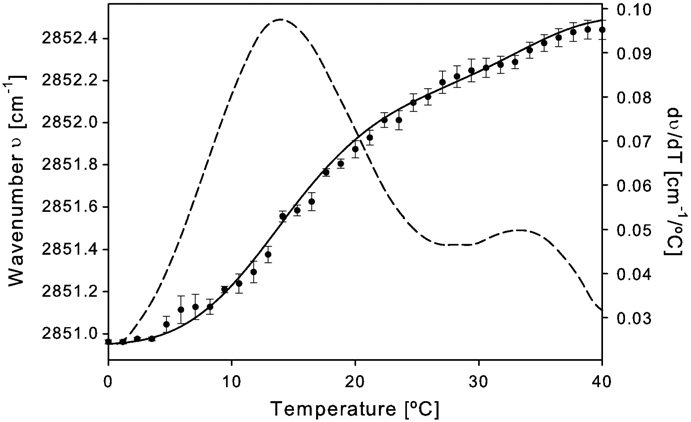
\includegraphics[scale=0.3]{transicion.png}
  \caption{ N\'{u}mero de onda de la banda de CH$_{2}$ en funci\'{o}n de la temperatura y su derivada para la membrana de \textit{S. aureus}. Imagen tomada de \cite{Ocampo2010TheAureus}.}
  \label{fig:ent2}
\end{figure}
En la figura \ref{fig:ent2} cabe destacar que el n\'{u}mero de onda es directamente proporcional a la energ\'{i}a de vibraci\'{o}n de las mol\'{e}culas debido a la relaci\'{o}n $E=h\nu$ con $\nu$ la frecuencia de vibraci\'{o}n.\\
La gr\'{a}fica \ref{fig:ent2} se obtuvo mediante la t\'{e}cnica de espectroscop\'{i}a de FITR variando la temperatura de la muestra.
\subsection{Espectrofot\'{o}metro de transformada de Fourier en el infrarrojo (FTIR)}
Es un instrumento basado en el interfer\'{o}metro de Michelson cuyo objetivo es medir el espectro de absorci\'{o}n y/o de emisi\'{o}n de una muestra en el infrarrojo. En el espectrofot\'{o}metro dos haces policrom\'{a}ticos  toman diferentes caminos \'{o}pticos. La diferencia de fases es una medida de la intensidad de luz que sale de la muestra. La idea de producir la diferencia de fases es que uno de los haces pase por la muestra. Se llama (IR) de rayos infrarrojos porque el barrido de longitudes de onda que hace el espectrofot\'{o}metro es sobre el infrarrojo.
En la figura \ref{fig:FTIR} se muestra el esquema de un FTIR la cual se discute a continuaci\'{o}n.
\begin{figure}[h]
  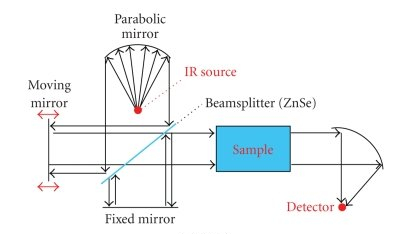
\includegraphics[width=\linewidth]{FTIR.jpg}
  \caption{Esquema de un FTIR. Figura tomada de \cite{Downes2010}.}
  \label{fig:FTIR}
\end{figure}
\subsection{Curvas de Crecimiento}
Con el fin de medir las transiciones de fase, se desea buscar el punto \'{o}ptimo en el cual la poblaci\'{o}n de c\'{e}lulas vivas sea mayor a la de c\'{e}lulas muertas y adem\'{a}s nos encontremos cerca del equilibrio poblacional.\\
Desde el siglo XIX es bien conocido que una poblaci\'{o}n bacteriana sigue cuatro fases \cite{Unknowna} denominadas \textit{fase de adaptaci\'{o}n} (lag),  \textit{fase exponencial},  \textit{fase de estacionaria} y muerte celular o fase de decrecimiento logar\'{i}tmico. Las primeras tres fases se han modelado mediante la ecuaci\'{o}n log\'{i}stica \cite{Zill2009} que tiene en cuenta el crecimiento exponencial y la competencia. La soluci\'{o}n de la ecuaci\'{o}n log\'{i}stica en este caso es una curva sigmoidal de la forma:
\begin{equation}
    P(t)=\frac{aP_{0}}{bP_{0}+(a-bP_{0})e^{-at}},
\end{equation}\label{eq:2}
donde $P(\infty)=a/b$
Una curva de crecimiento tiene la forma mostrada en la figura .
\begin{figure}[h]
  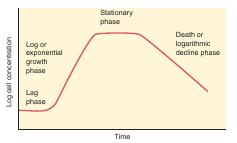
\includegraphics[width=\linewidth]{curva.png}
  \caption{Fases de una curva de crecimiento en escala log. Las primeras tres fases se modelan como una sigmoidal. Figura tomada de \cite{Unknowna}.}
  \label{fig:curv}
\end{figure}
\section{\label{sec:exp}Marco Experimental}
Para estudiar la transici\'{o}n de fase s\'{o}lido-ordenado/l\'{i}quido-desordenado de la membrana de \textit{S. aureus} en presencia y ausencia de estafiloxantina se plantea obtener gr\'{a}ficas de posici\'{o}n de la banda CH$_{2}$ sim\'{e}trico en funci\'{o}n de la temperatura.

\subsection{Curva de Crecimiento}
Se toman tres cepas de \textit{S. aureus}, la nativa llamada
144, una  que es un mutante (knockout) del gen crtM de la ruta
de s\'{i}ntesis de estafiloxantina(no produce estafiloxantina) llamada 145 y una que mediante un pl\'{a}smido con el gen crtM produce un exceso de carotenoides,llamada 147. A las tres cepas se les realiza una curva de crecimiento. Esto se realiza con el fin de conocer cual es la fase estacionaria
de la curva que va a ser el punto \'{o}ptimo de trabajo.\\

Para dicha tarea se recuperan las c\'{e}lulas que est\'{a}n a -80\textdegree C, es decir, se toma una colonia y se cultivan en cajas Petri que contienen LB-agar, figura \ref{fig:curv1} paso 1). Como la 147 tiene el pl\'{a}smido al LB-agar debe agreg\'{a}rsele 1$\mu$g/$m$L del antibi\'{o}tico eritromicina para que el pl\'{a}smido quede dentro de la bacteria. El valor de la concentraci\'{o}n \'{o}ptima de eritromicina se determin\'{o} mediante un experimento previo, ver figura \ref{fig:144_eri} y documento del avance. En dicho experimento se realizan curvas de crecimiento de la cepas 144  y 147 encontr\'{a}ndose que a partir de 1$\mu$g/$m$L de eritromicina hay crecimiento de las cepas.\\

Luego se toma una colonia de cada caja Petri, se diluye en 10mL de LB l\'{i}quido y se deja en overnight dentro del agitador ``Shaker'' a  37\textdegree C, ver figura \ref{fig:curv1} paso 3).\\

 Al tomar una gota de la diluci\'{o}n dejada en overnight, se puede conocer el n\'{u}mero de c\'{e}lulas contenidas en la gota usando el nanodrop o un espectrofot\'{o}metro, el n\'{u}mero de c\'{e}lulas ser\'{a} proporcional a la absorbancia, \ref{fig:curv1} paso 4).\\
\begin{figure}
 \input{./Imagenes/esquema1.pdf_tex}
  \input{./Imagenes/nanodrop.pdf_tex}
  \caption{Pasos para realizar una curva de crecimiento. 1) Recuperaci\'{o}n de c\'{e}lulas a cajas petri con LB. 2) Diluci\'{o}n colonia a LB l\'{i}quido. 3) Frasco diluido a Shaker 4) Medici\'{o}n de absorbancia con nanodrop. }
  \label{fig:curv1}
\end{figure}
\begin{figure}[h]
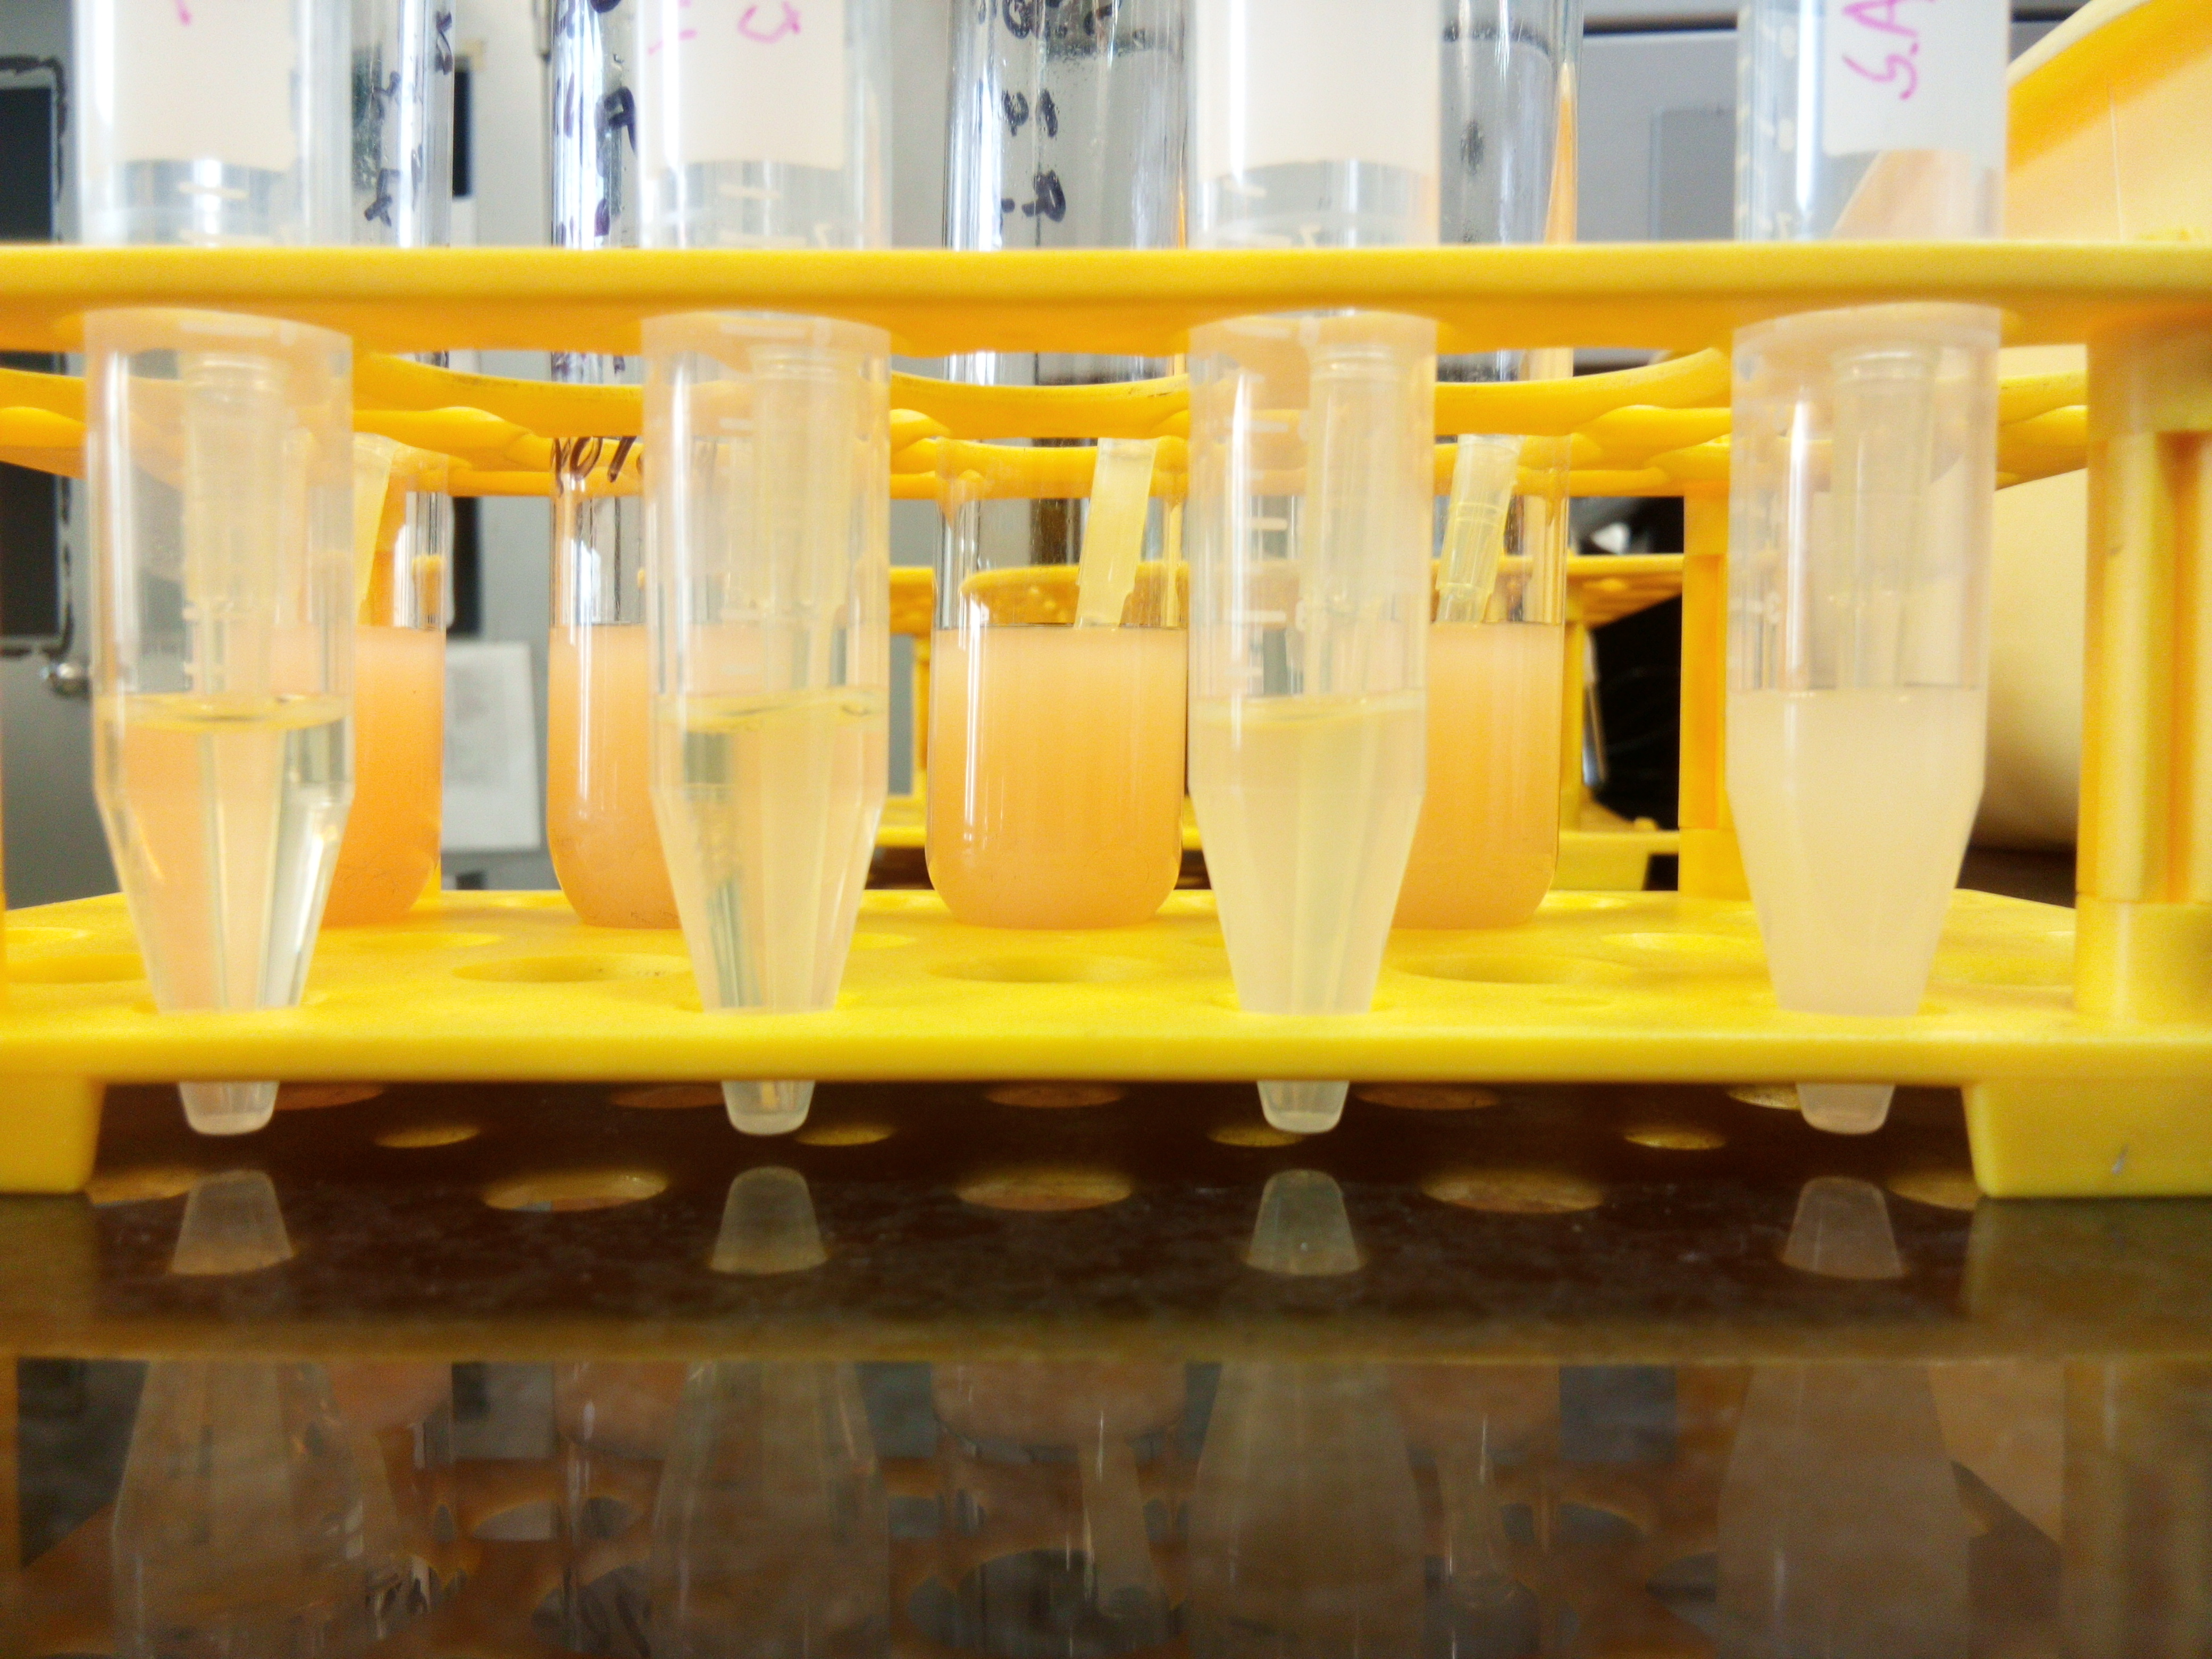
\includegraphics[scale=0.04]{./Imagenes/144_eri.jpg}
  \caption{Crecimiento de la cepa 144 con diferentes concentraciones de  eritromicina. De derecha a izquierda 0.4$\mu$g/mL, 0.8$\mu$g/mL, 1$\mu$g/mL y 1.2$\mu$g/mL de  eritromicina.}
  \label{fig:144_eri}
\end{figure}
 \subsection{Espectro FTIR}
Antes de trabajar con un sistema \textit{in vivo} se miden los espectros para liposomas hechos de  DMPC (dimiristoil fosfatidilcolina) en funci\'{o}n de la temperatura, esto en parte para verificar el funcionamiento del control de temperatura y en parte como comparaci\'{o}n del sistema modelo al vivo. El control de temperatura tiene un encapsulado cuyo interior tiene una l\'{a}mina de Cu que calienta la muestra y vidrios de Ge transparentes al infrarrojo. En el centro de las dos l\'{a}minas de Ge se coloca la muestra.  La temperatura se variar\'{a} por debajo de la temperatura ambiente (aproximadamente desde 10\textdegree C) y por encima de la temperatura ambiente ( abajo de 40\textdegree C aproximadamente) en pasos de a 5 \textdegree C cada minuto, ver \cite{Ocampo2010TheAureus}. Para tomar el espectro por cada temperatura se acopla el control de temperatura al FTIR, tal como se ilustra en la figura \ref{fig:mont2}.\\
\begin{figure}
 \input{./Imagenes/esquema2.pdf_tex}
  \caption{Esquema del control de temperatura acoplado al FTIR usado para medir el espectro en funci\'{o}n de la temperatura.}
  \label{fig:mont2}
\end{figure}
Una vez trabajado los liposomas de DPPC\footnote{Liposomas proporcionados por el grupo de biof\'{i}sica}, se mide el espectro de las tres cepas 144, 145 y 147. Para esto, debe tenerse en cuenta la curva de crecimiento. Con la curva se establece el punto de crecimiento \'{o}ptimo de las c\'{e}lulas a trabajar. Una vez escogido este punto, se coloca una muestra de \textit{S. aureus} en el interior del control de temperatura \footnote{Mediciones realizadas con la colaboraci\'{o}n del grupo de qu\'{i}mica arom\'{a}tica de la universidad},  y se miden los espectros para cada temperatura tal como se describi\'{o} antes.
Se busca en la curva del espectro de absorbancia el pico correspondiente a la vibraci\'{o}n asim\'{e}trica de CH$_{2}$ el cual est\'{a} alrededor de $2853 \mathrm{cm}^{-1}$ y se mide el valor del n\'{u}mero de onda de este pico en funci\'{o}n de la temperatura. La temperatura es el par\'{a}metro controlable mediante la interfaz que conecta al computador.
\section{Resultados Preliminares y An\'alisis}
Las curvas de crecimiento obtenidas para las cepas 144 y 145 son las mostradas en la gr\'{a}fica \ref{fig:cur1}. Las densidades \'{o}pticas en funci\'{o}n del tiempo para la 144 y la 145 (d\'{i}a 1) son la verde y la roja respectivamente; estas fueron tomadas hasta que se visualizara un cambio de concavidad en las curvas, lo cual ocurri\'{o} alrededor de las 12 horas. Los puntos m\'{a}s altos que est\'{a}n al inicio representan los valores de la densidad \'{o}ptica del overnight. Se espera que las curvas alcancen este valor de la densidad \'{o}ptica cuando lleguen a la fase estacionaria. La curva de la cepa 147 se intent\'{o} realizar pero no creci\'{o}.\\
\begin{figure}[h]
 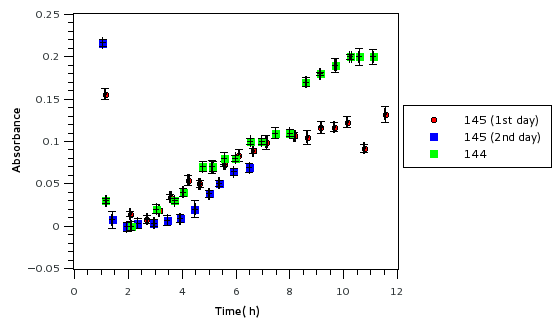
\includegraphics[width=\linewidth]{curvas/gratodas.png}
  \caption{Curvas de crecimiento para las cepas 144 y 145}
  \label{fig:cur1}
\end{figure}
 A pesar de que la cepa 145 se cultiv\'{o} en cloranfenicol, se esperaba que esta tuviera un tiempo de adaptaci\'{o}n (lag phase) m\'{a}s prolongado que el de la 144 ya que la cepa 145 no produce carotenoides. Con base en esto, se decide tomar nuevamente los datos de la curva 145, representada en la gr\'{a}fica  \ref{fig:cur1} como 145 (d\'{i}a 2) en azul. Se observa que la 145 (d\'{i}a 2) tiene un tiempo de adaptaci\'{o}n m\'{a}s prolongado que la 145 (d\'{i}a 1) y en general que su curva de crecimiento es menor a las otras dos.\\
 
 Para las cepa 144, 145 (d\'{i}a 1) y 145 (d\'{i}a 2) se realiza un ajuste a la sigmoidal \eqref{eq:2}\\
 Para la 144 se encontr\'{o} un coeficiente de determinaci\'{o}n de $r^2=0.784$. Los valores $a$, $b$ y $P_{0}$ de la sigmoidal ajustados se discutir\'{a}n en la en informe final.
\begin{figure}[h]
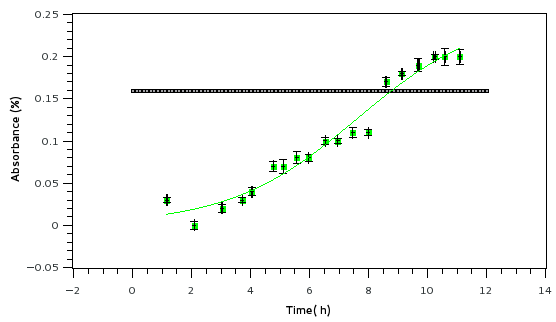
\includegraphics[width=\linewidth]{curvas/gra144.png}
  \caption{Curva de crecimiento para las cepas 144, 145 y 147}
  \label{fig:cur2}
   Para la 145  (d\'{i}a 1) se encontr\'{o} un coeficiente de determinaci\'{o}n de $r^2=0.994$.
   Los valores $a$, $b$ y $P_{0}$ de la sigmoidal ajustados se discutir\'{a}n en la en informe final.
\end{figure}
\begin{figure}[h]
 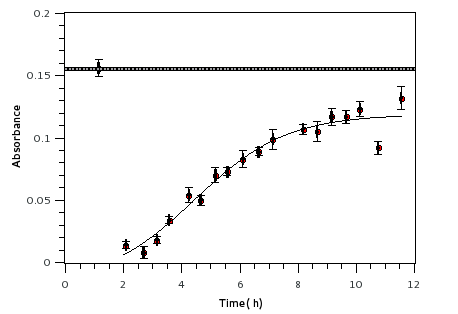
\includegraphics[width=\linewidth]{curvas/gra145dia1.png}
  \caption{Curvas de crecimiento para las cepas 144, 145 y 147}
  \label{fig:cur3}
\end{figure}
 Para la 145  (d\'{i}a 2) se encontr\'{o} un coeficiente de determinaci\'{o}n de $r^2=0.955$. 
 Los valores $a$, $b$ y $P_{0}$ de la sigmoidal ajustados se discutir\'{a}n en la en informe final.
\begin{figure}[h]
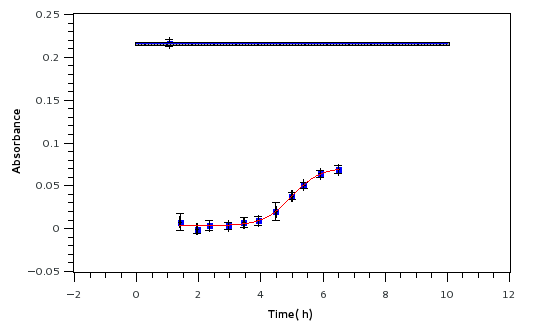
\includegraphics[width=\linewidth]{curvas/gra145dia2.png}
  \caption{Curvas de crecimiento para las cepas 144, 145 y 147}
  \label{fig:cur4}
\end{figure}
Debido a que la cepa 147 no creci\'{o} en antibi\'{o}tico se realiza otro experimento en el cual crece \textit{S. aureus} cepas 144 y 147 diluidas en LB a diferentes concentraciones de antibi\'{o}tico, esto con el fin de determinar la concentraci\'{o}n adecudad de antib\'{o}tico suministrado a la 147. Se preparan 5 frascos con c\'{e}lulas 144, 5 con 147 y a cada frasco se le agregan diferentes concentraciones de eritromicina 0.4$\mu$g/mL, 0.8$\mu$g/mL, 1$\mu$g/mL, 1.2$\mu$g/mL y 1.4$\mu$g/mL y se dejan en el agitador (shaker) entre 4 y 6 horas \footnote{Este experimento fue realizado por el equipo del laboratorio de biof\'{i}sica}\\
Los resultados obtenidos para el experimento fueron los mostrados en la figura \\
De la figura \ref{fig:144_eri} se puede concluir que la concentraci\'{o}n de eritromicina m\'{a}s adecuada para crecer la cepa 147 es de 1$\mu$g/mL.
\subsection{Espectro en funci\'{o}n de la Temperatura}
Para bicapas compuestas por DPPC se obtienen los espectros a 13\textdegree C, 17\textdegree C, 20\textdegree C, 25\textdegree C, 30\textdegree C y 35\textdegree C mostrados en el anexo. En la figura \ref{fig:espa13} se muestran los dos valles de inter\'{e}s para $T=13$\textdegree C.
\begin{figure}[h]
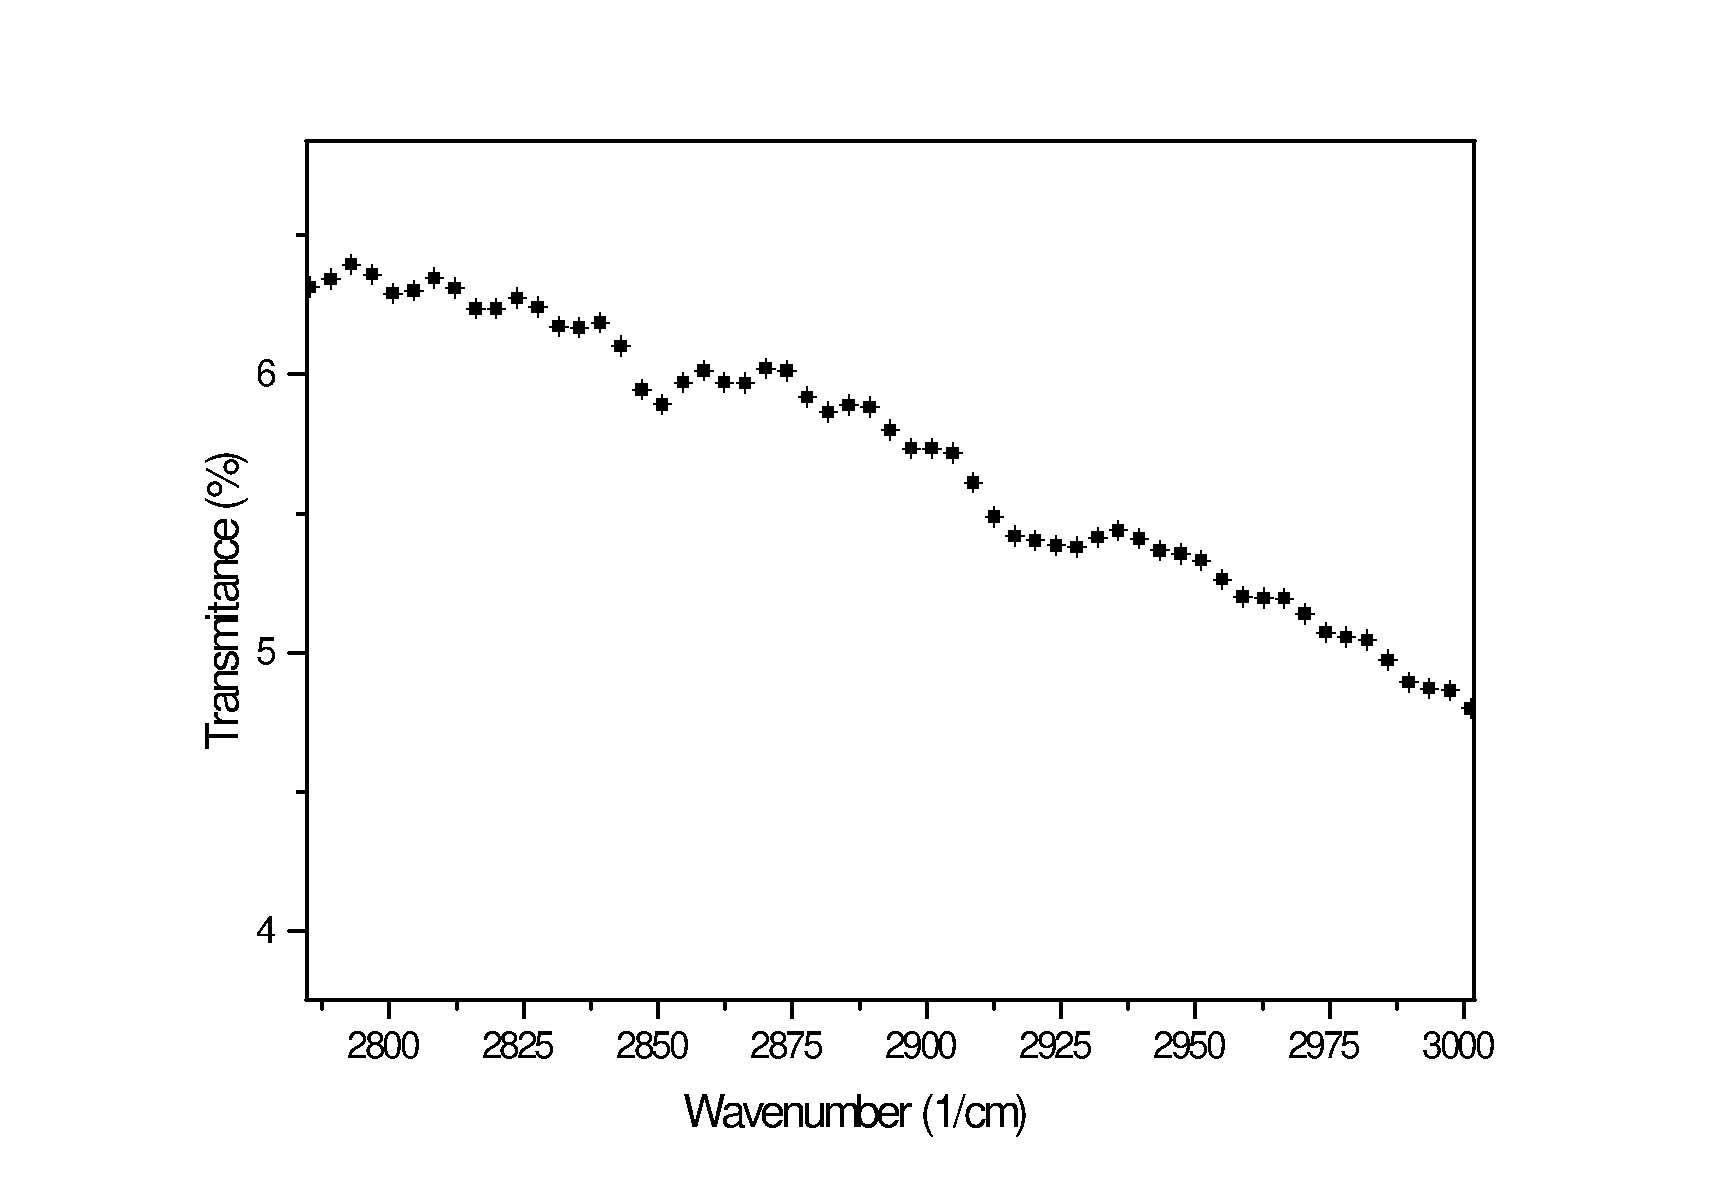
\includegraphics[scale=0.3]{FTIR/13C.pdf}
  \caption{Regi\'{o}n del espectro de absorci\'{o}n para DPPC entre 2780 cm $^{-1}$ y 3000 cm $^{-1}$ a $T=13$\textdegree C.}
  \label{fig:espa13}
\end{figure}
Con el fin de conocer los valores experimentales de estos valles (que en adelante los llamaremos picos si consideramos el inverso del espectro de absorci\'{o}n) primero se calcula el inverso multiplicativo del espectro y luego se hallan mediante el m\'{e}todo de la segunda derivada en $Qtiplot$. En la tabla 1 se muestran los valores y las posiciones de los picos encontrados para las 6 temperaturas:
\begin{table}[h]
    \centering
    \begin{tabular}{|c|c|}
         $(T\pm 1)$\textdegree C & $(k\pm 1\times 10^{-6}$cm$^-1$ \\\hline
        13 & 2850.790048\\
  17 & 2862.362944\\
  20&2862.362944\\
 25 &2877.793472\\
    \end{tabular}
    \caption{Número de onda del primer pico de la izquierda( Ver figuras 15 a 19 del anexo) para cada una de las temperaturas.}
    \label{tab:knumb}
\end{table}

De la tabla se observa que aunque hay un aumento en la temperatura de 20\textdegree C a 25\textdegree C tambi\'{e}n existe esta variaci\'{o}n al pasar de 13\textdegree C a 17\textdegree C. Estas variaciones pueden deberse a  que el espectro presenta unas interferencias que pueden modificar los picos, estas son las ondulaciones mostradas en la gr\'{a}fica \ref{fig:espa13}. Las interferencias son causadas por sitio dende se coloca la muestra en el control de temperatura.
%%%%%%%%%%%%%%%%%%%%%%%%%%%%%%%%%%%%%%%%%%%%%%%%%%%%%%%
\section{Conclusiones y Trabajo Futuro Documento}
De las gr\'{a}ficas para las curvas de crecimiento \ref{fig:cur1} se encuentra que a pesar de que los tiempos de crecimiento para la 145 no son los esperados, tanto para la 144 como para la 145 se observa un crecimiento con la forma de una curva sigmoidal.\\
Debido a que la cepa 147 no mostr\'{o} crecimiento bajo las condiciones dadas en el marco experimental y a que la cepa 145 mostr\'{o} diferencias para los dos d\'{i}as, se realizar\'{a}n nuevamente las curvas de crecimiento para todas las cepas teniendo en cuenta que la concentraci\'{o}n de eritromicina que se suministrar\'{a} a las cepas 145 y 147 ser\'{a} de 1$\mu$g/mL.\\
En cuanto a los espectros aunque se observa un aumento en el n\'{u}mero de onda contra la temperatura no se puede distinguir claramente la transici\'{o}n de fase de los liposomas hechos de DPPC. Se ha trabajado en disminuir la interferencia para encontrar encontrar el aumento abrupto en los picos alrededor de $23-24$ \textdegree C y se ya se ha disminuido la interferencia (resultados no mostrados aqu\'{i}). Como ya se logr\'{o} disminuir la intererencia se pasar\'{a} a medir los espectros en funci\'{o}n de la temperatura para las cepas 144, 145 y 147 de \textit{S. aureus} vivas.\\

\begin{acknowledgments}
We wish to acknowledge the support of the author community in using
REV\TeX{}, offering suggestions and encouragement, testing new versions,
\dots.
\end{acknowledgments}

\appendix
\section*{Anexo: Espectros obtenidos por FTIR para membranas de DPPC}
\begin{figure}[ht]
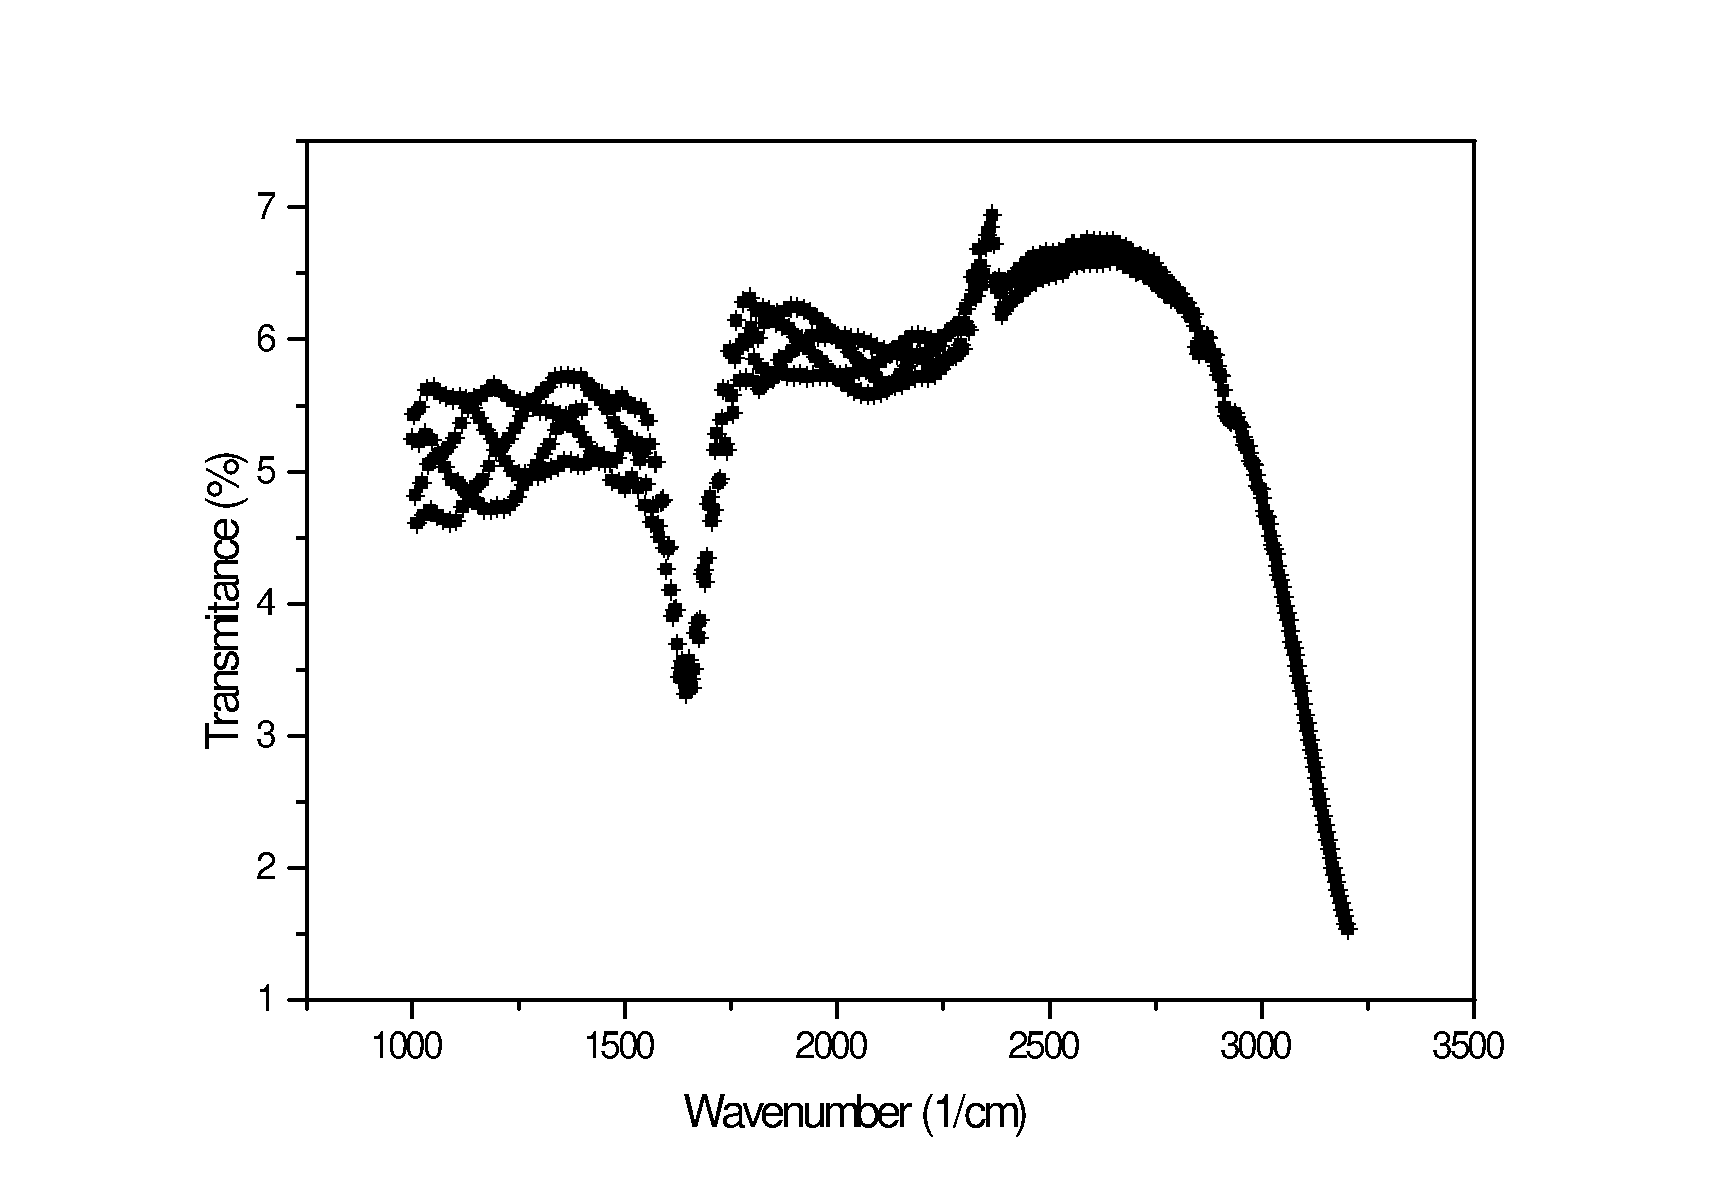
\includegraphics[scale=0.2]{FTIR/Graph1.pdf}
  \caption{Espectro de absorci\'{o}n para DPPC entre 1000 cm $^{-1}$ y 3300 cm $^{-1}$ a $T=13$\textdegree C.}
  \label{fig:13}
\end{figure}
\begin{figure}[ht]
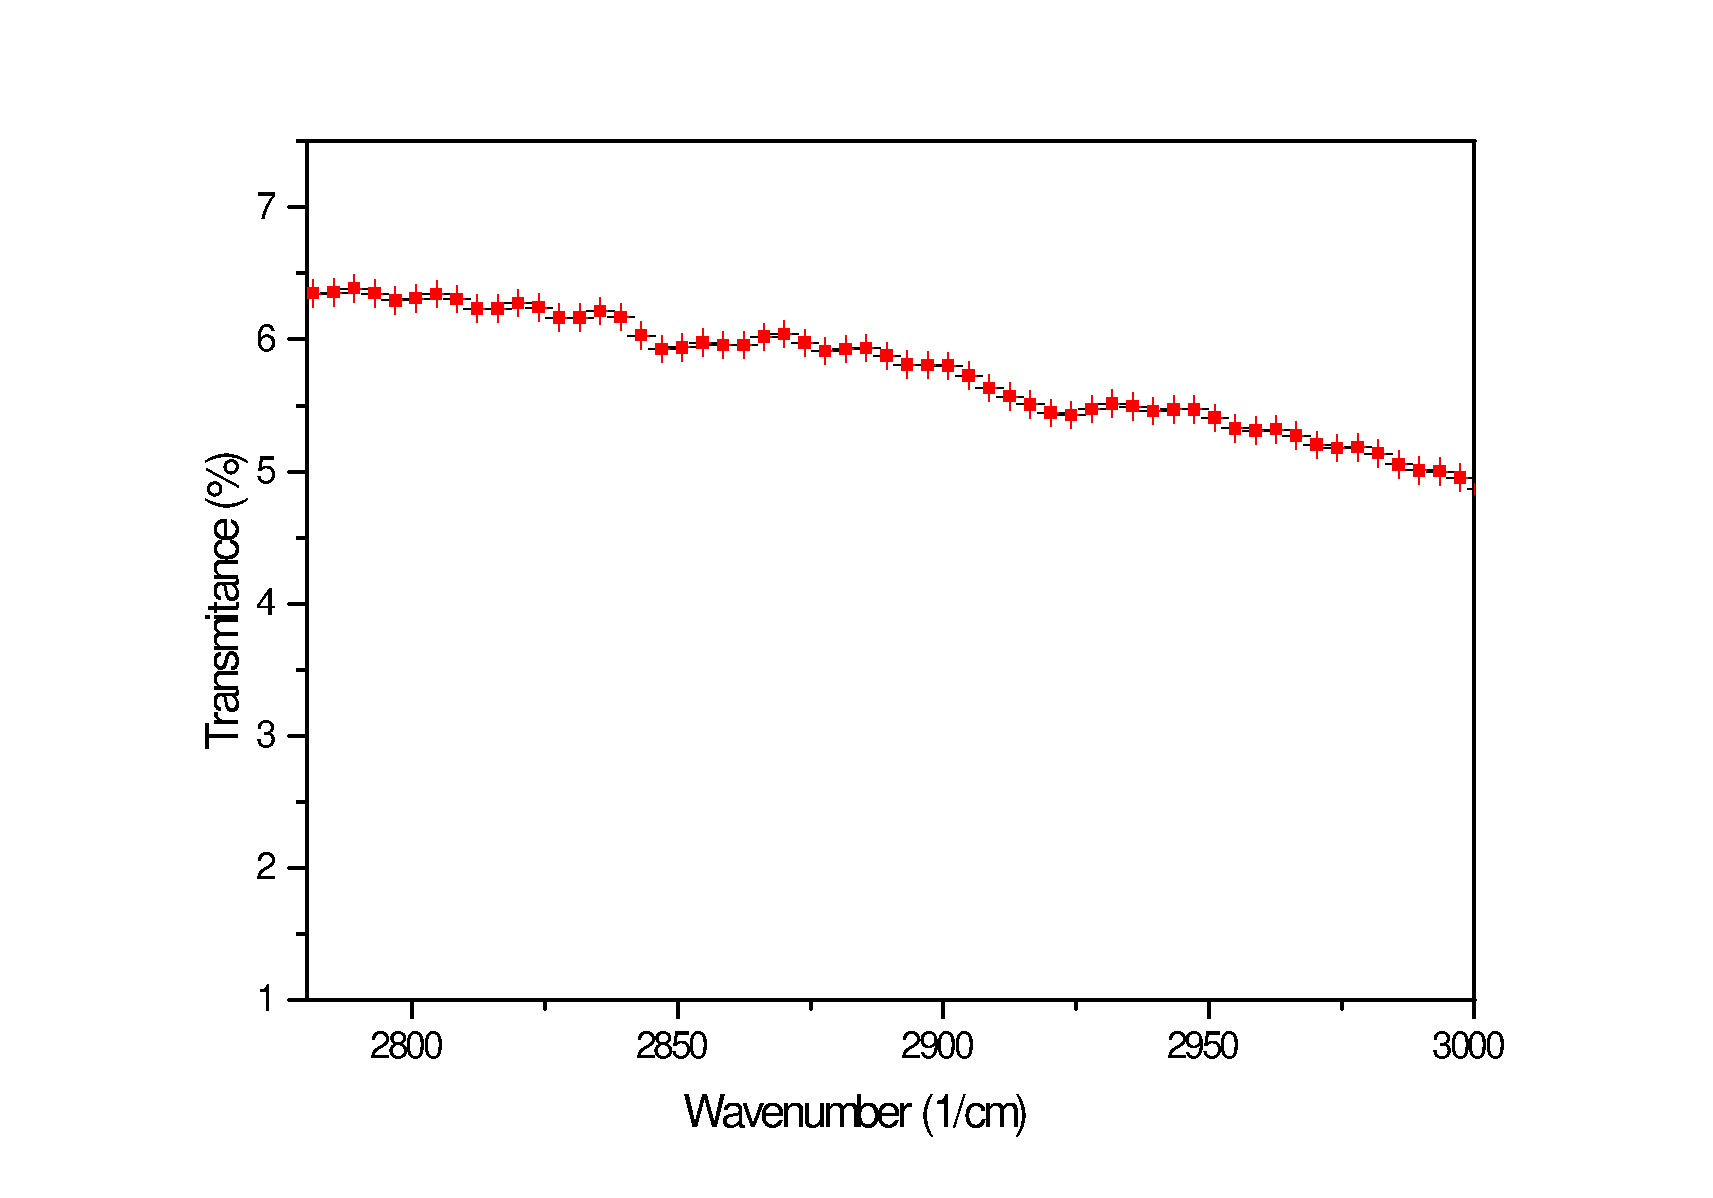
\includegraphics[scale=0.25]{FTIR/17C.pdf}
  \caption{Regi\'{o}n del espectro de absorci\'{o}n para DPPC entre 2780 cm $^{-1}$ y 3000 cm $^{-1}$ a $T=17$\textdegree C.}
  \label{fig:espa17}
\end{figure}
\begin{figure}[ht]
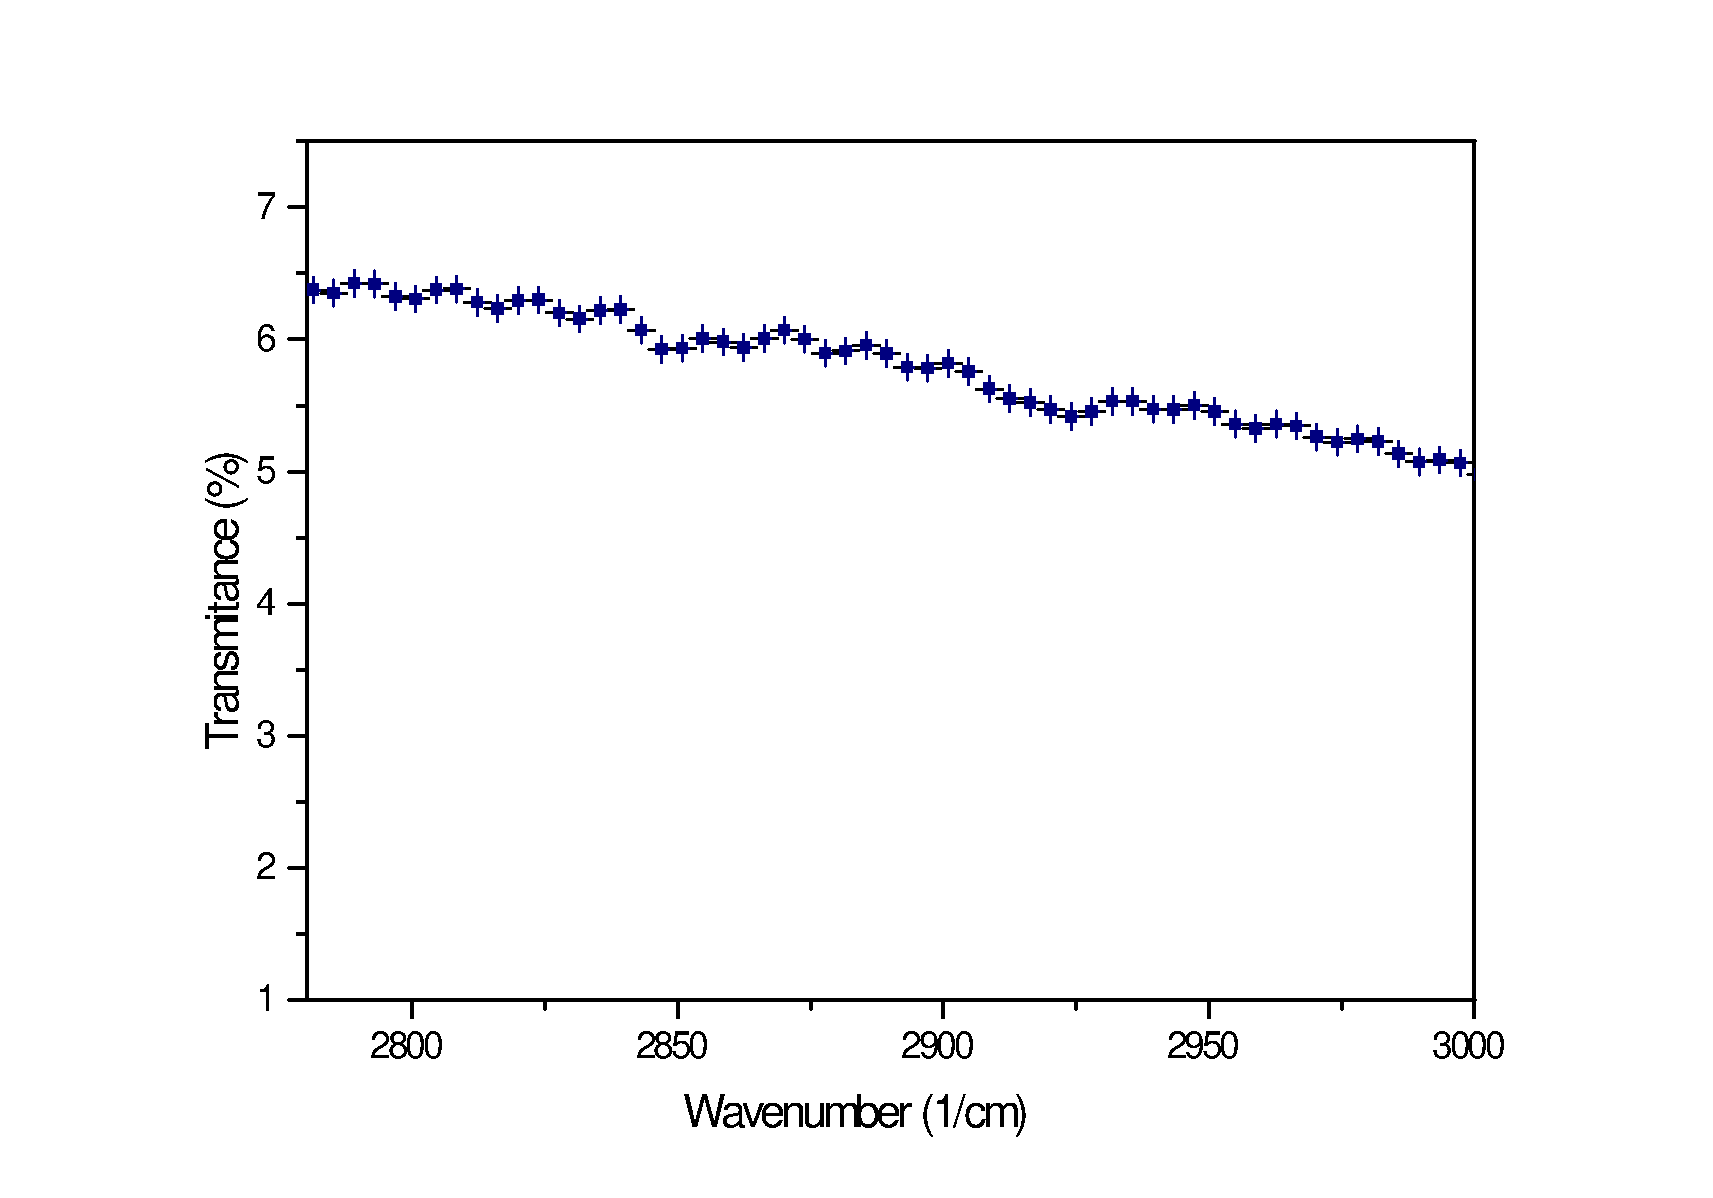
\includegraphics[scale=0.25]{FTIR/20C.pdf}
  \caption{Regi\'{o}n del espectro de absorci\'{o}n para DPPC entre 2780 cm $^{-1}$ y 3000 cm $^{-1}$ a $T=20$\textdegree C.}
  \label{fig:espa20}
\end{figure}
\begin{figure}[ht]
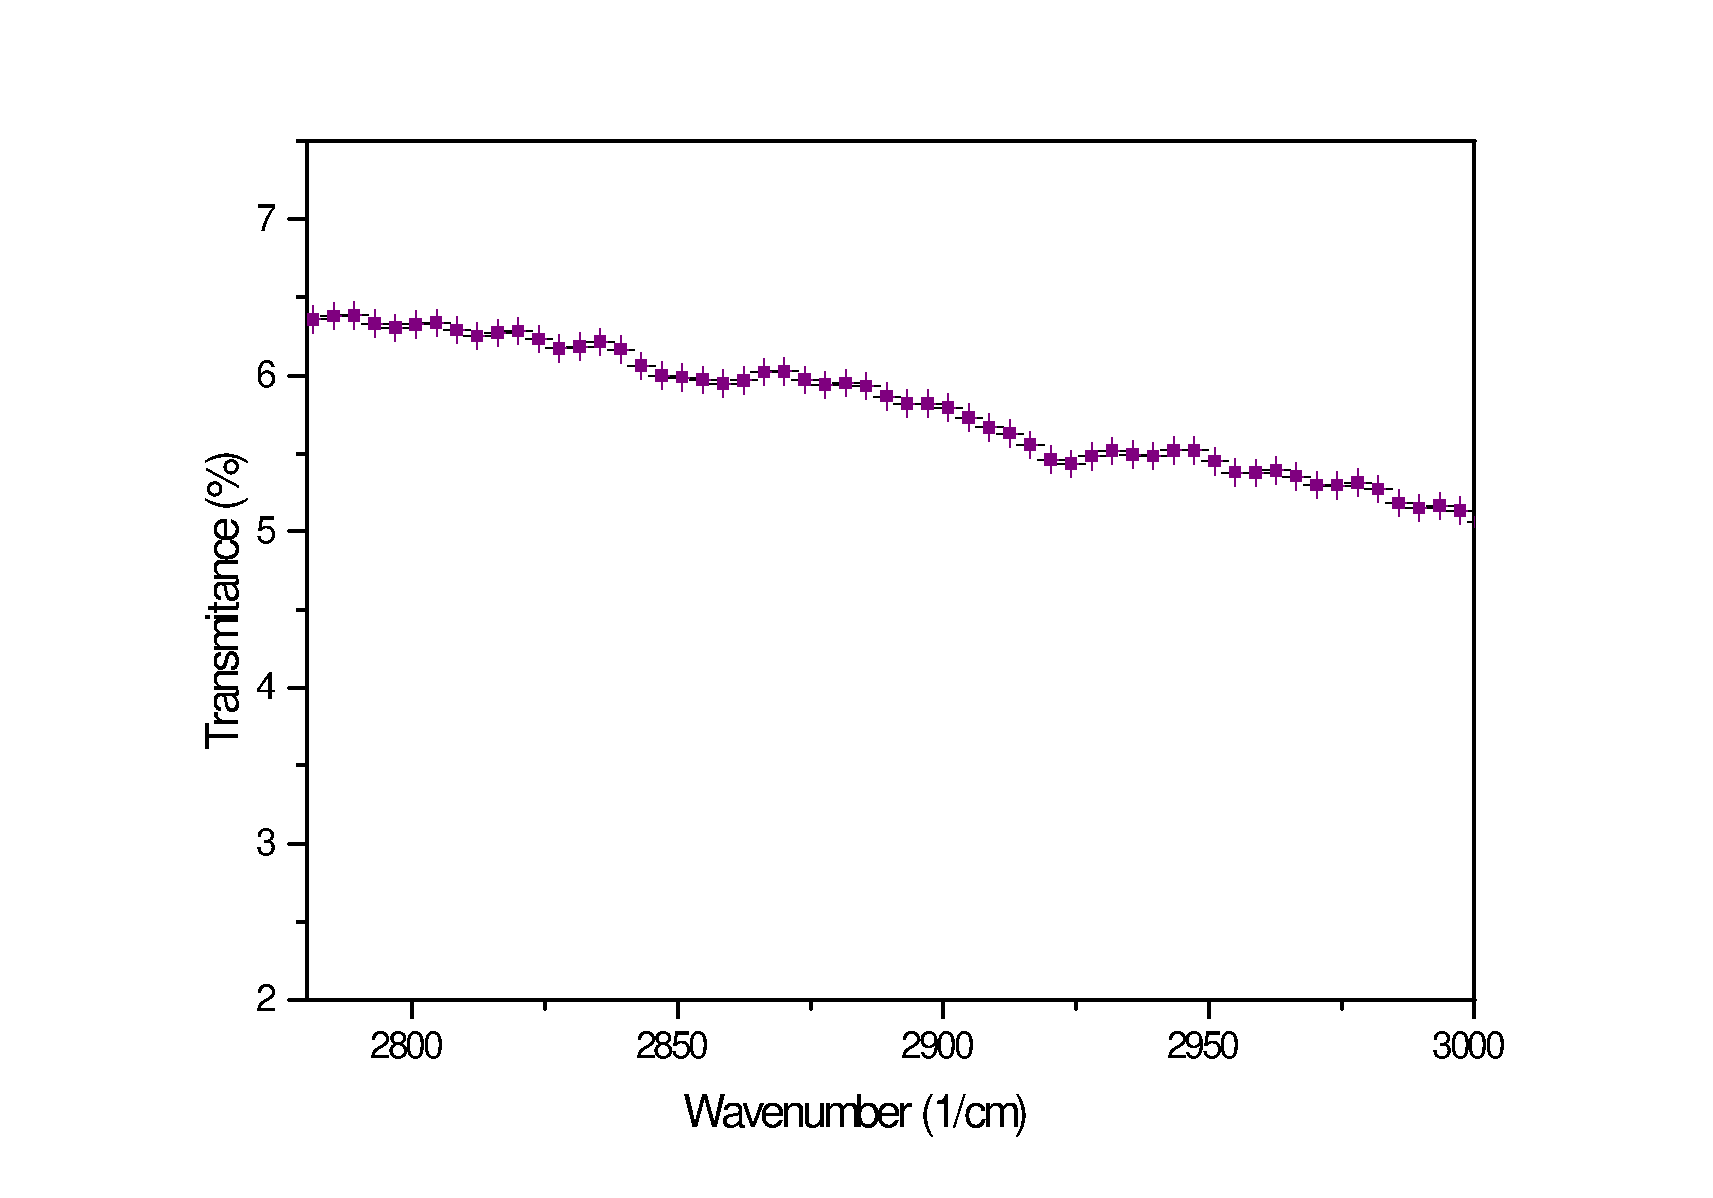
\includegraphics[scale=0.25]{FTIR/25C.pdf}
  \caption{Regi\'{o}n del espectro de absorci\'{o}n para DPPC entre 2780 cm $^{-1}$ y 3000 cm $^{-1}$ a $T=25$\textdegree C.}
  \label{fig:espa25}
\end{figure}
\begin{figure}[ht]
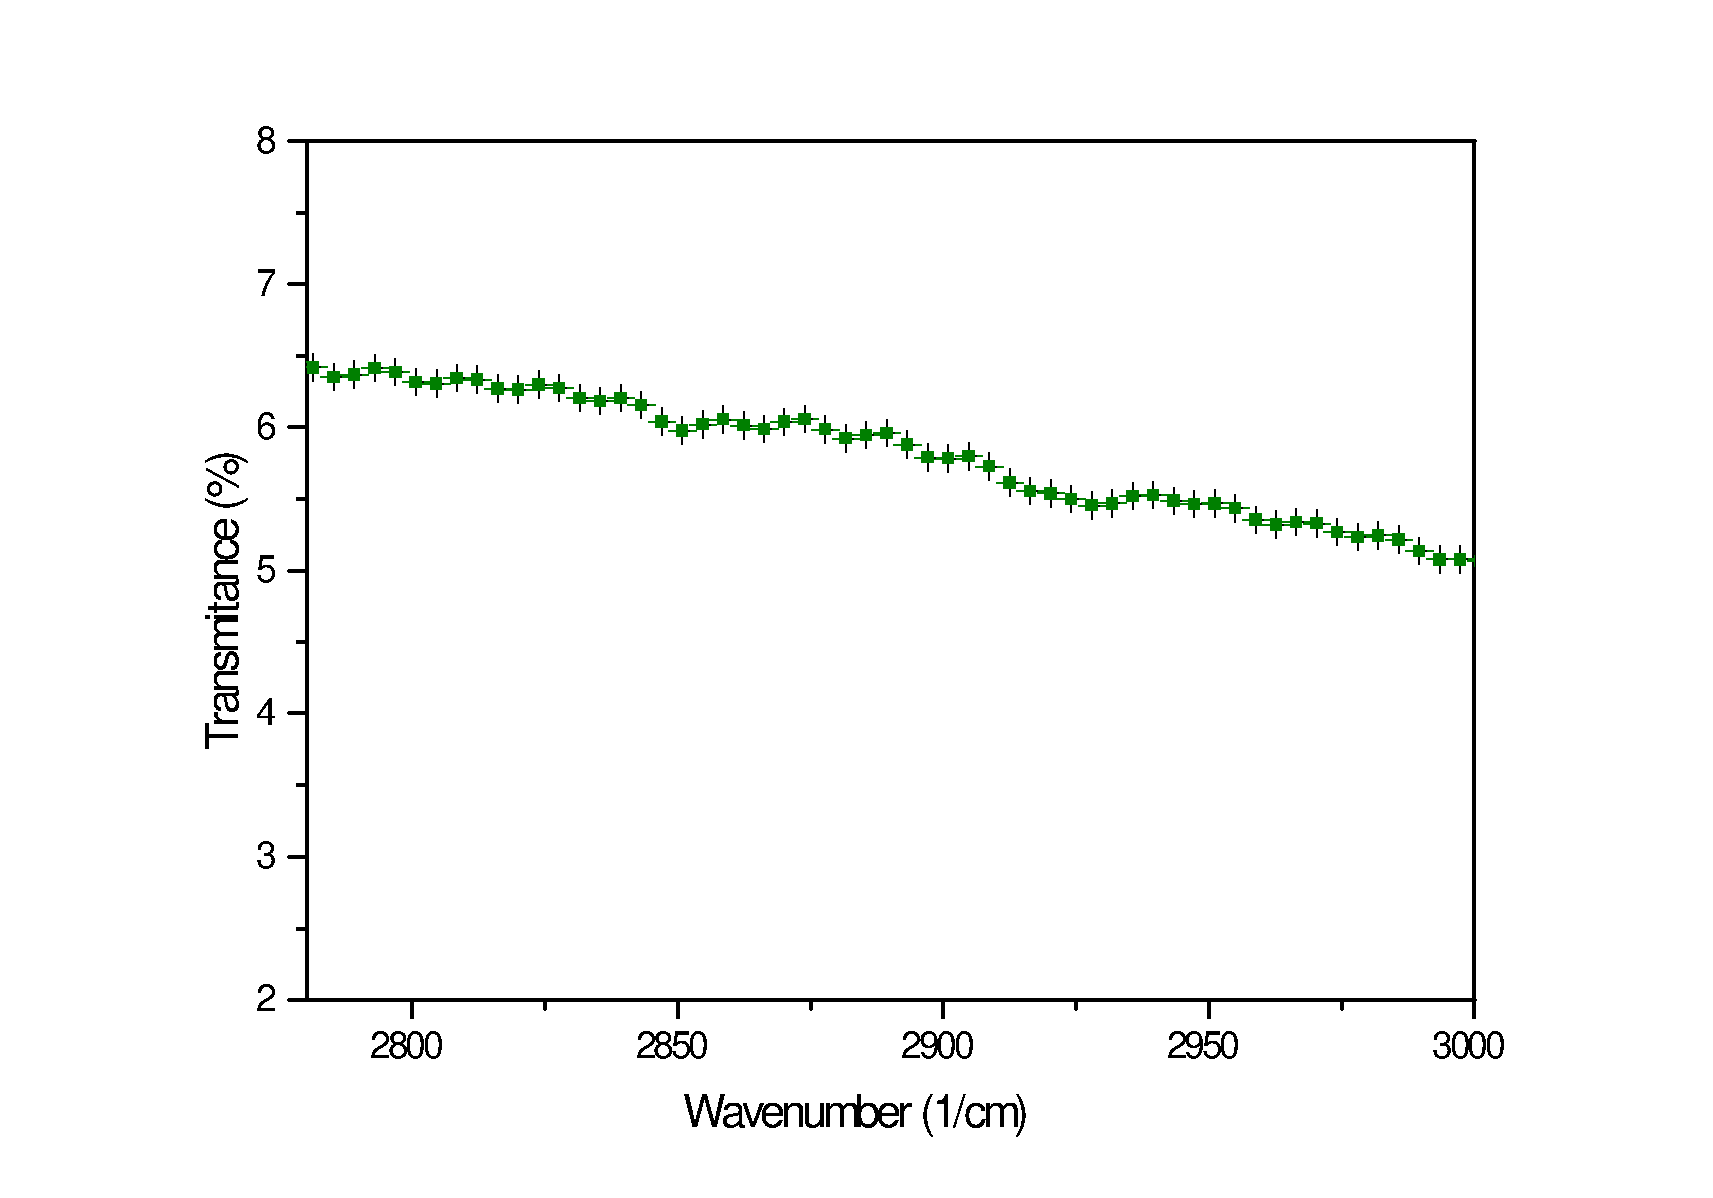
\includegraphics[scale=0.25]{FTIR/30C.pdf}
  \caption{Regi\'{o}n del espectro de absorci\'{o}n para DPPC entre 2780 cm $^{-1}$ y 3000 cm $^{-1}$ a $T=30$\textdegree C.}
  \label{fig:espa30}
\end{figure}
\begin{figure}[ht]
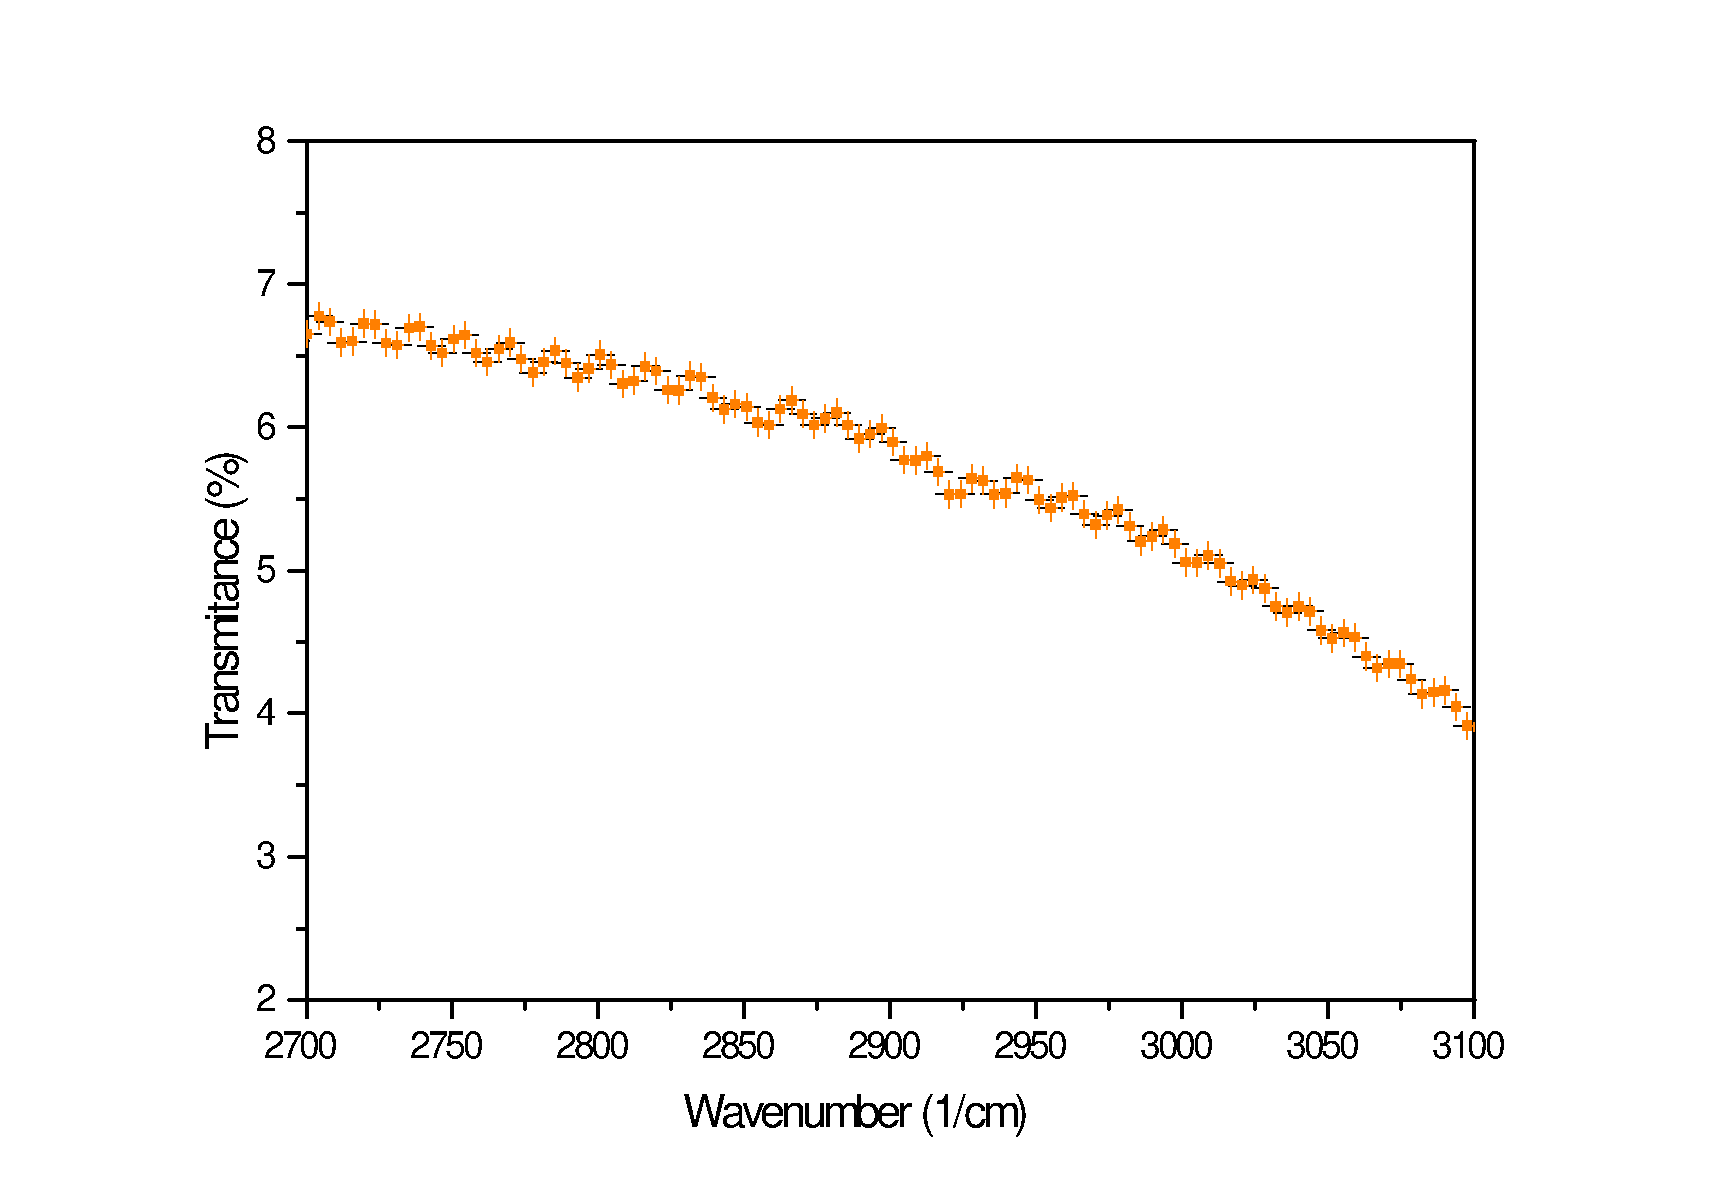
\includegraphics[scale=0.25]{FTIR/35C.pdf}
  \caption{Regi\'{o}n del espectro de absorci\'{o}n para DPPC entre 2780 cm $^{-1}$ y 3000 cm $^{-1}$ a $T=35$\textdegree C.}
  \label{fig:espa35}
\end{figure}

% The \nocite command causes all entries in a bibliography to be printed out
% whether or not they are actually referenced in the text. This is appropriate
% for the sample file to show the different styles of references, but authors
% most likely will not want to use it:
%\nocite{*}

\bibliography{references}% Produces the bibliography via BibTeX.

\end{document}
%
% ****** End of file apssamp.tex ******
